% This will be the main document for the Technical Networks paper to
% be written by the Eggnet team of Jordan Ell, Triet Huynh and Braden
% Simpson in association with Adrian Schroeter and Daniela Damian.

\documentclass[conference]{IEEEtran}

% Use of outside images
\usepackage{graphicx} 
% Use text inside euqations
\usepackage{amsmath}

\usepackage{balance}
\usepackage{float}
\usepackage{caption}
\floatstyle{plaintop}
\restylefloat{table}

% Correct bad hyphenation here
\hyphenation{op-tical net-works semi-conduc-tor}

% Begin the paper here
\begin{document}


% Paper title
% Can use linebreaks \\ within to get better formatting as desired
\title{Review: Exploring Multi-Threaded Java Application Performance on Multicore Hardware}

% Authors names
\author{\IEEEauthorblockN{Jordan Ell and Braden Simpson}
\IEEEauthorblockA{University of Victoria,
Victoria, British Columbia, Canada \\ jell, braden\{@uvic.ca\}}
}

% Make the title area
\maketitle

\begin{abstract}
The actual paper's abstract for reference: While there have been many studies of how to schedule applications to take advantage of increasing numbers of cores
in modern-day multicore processors, few have focused on
multi-threaded managed language applications which are
prevalent from the embedded to the server domain. Managed
languages complicate performance studies because they
have additional virtual machine threads that collect garbage
and dynamically compile, closely interacting with application threads. Further complexity is introduced as modern
multicore machines have multiple sockets and dynamic frequency scaling options, broadening opportunities to reduce
both power and running time.
In this paper, we explore the performance of Java applications, studying how best to map application and virtual machine (JVM) threads to a multicore, multi-socket environment. We explore both the cost of separating JVM threads
from application threads, and the opportunity to speed up or
slow down the clock frequency of isolated threads. We perform experiments with the multi-threaded DaCapo benchmarks and pseudojbb2005 running on the Jikes Research
Virtual Machine, on a dual-socket, 8-core Intel Nehalem
machine to reveal several novel, and sometimes counterintuitive, findings. We believe these insights are a first but
important step towards understanding and optimizing managed language performance on modern hardware.
\end{abstract}

\section{Problem}
\label{sec:problem}

The problems being discussed by the authors in this paper mainly focus on the lack of 
experimental knowledge in the domain of multicore hardware and interpreted languages (
specifically threaded applications).
The authors begin with a focus on the fact that multicore hardware systems are becoming
more and more common and continuing to expand in the number of cores and sockets moving
into the future due to Moore's Law~\cite{Moore:2000:CMC}. The authors also explain that multicore performance
for most standard programming languages (non-interpreted) is a much studied field and
has been extensively tested. However, the domain of interpreted languages is still a largely
unstudied and untested domain when it comes to performance on multicore multisocket hardware
systems. This can be attributed to the fact that instead of having just application threads to
worry about, you have virtual machine threads which can pause application execution, be needed
prior to certain execution points, and otherwise trigger non-deterministic actions of the various threads.
This leads into various questions of what threads should be executed in isolation (if any) to
ensure proper caching, or which threads should be given a lower clock frequency.

This paper presents their exploratory approach of the problem domain as a novel understanding of 
the field. This paper focuses on several factors of multicore hardware running an interpreted
program in Java which are the following: the clock frequency of different type of execution threads; 
the isolation of different types of execution threads between both cores and sockets in the 
hardware; the isolation of different types of threads between cores and socket at different
execution times in the program; the pinning of different thread types to specific cores; and some
combined affects of the tests listed above. The types of threads listed above which are mentioned
specifically in the problems to be tested and the results are: garbage collection, compilation, 
all JVM threads, and all application threads.

To the authors knowledge, most of these experimental tests have not been studied in the past
except for the clock frequency or power implications of their research. Related work is mentioned
in that JVM services yield different performance and power characteristic compared to the Java
application itself. Other end-to-end performance test have been made in the field, however,
these tests were limited to single socket hardware. It has also been shown that the JVM
services consume on average 20\% of total power needed~\cite{Cao:2012:YYP}. The previous works show that the
domain of power designation inside of interpreted languages is very much a vital field
that should be researcher. 

The authors go on to explain
the importance of energy and power controls have, especially with regards to hand held devices.
The paper presents the idea of dark silicon which is the idea that high end servers will no longer
be able to power entire processors all the time. We believe this problem will soon be carried
over to the hand held market where battery life is becoming an increasing factor in the phone choice
of many consumers as phones become more powerful and require more energy to run. Intel's Turbo
Boost~\cite{Intel:2008} technology is a good representation of this problem as it allows for short duration 
clock frequency boosts on a limited number of cores.

In our opinion, the problems being investigated by this paper are extremely worthwhile when
it comes to any device with a limited processor speed or that is battery operated, and in the
case of mobile hardware, both. If the developers of Android can reduce power to an isolated
core on the phone which is in charge of running garbage collection to save 20\% processing
power, we believe this research will be of vital importance. Aside from 

\section{Methodology}

For the experimental tests, the authors consider multi-threaded test applications written in
Java. The authors also use a multicore, multisocket hardware configuration. The authors 
consider three main areas of focus (with combinations there of) which are: number of application
and JVM service thread; thread-to-core/socket mapping; and frequency scaling and power implications.
Through these three main areas of focus, 23 experiments are then preformed, each of which usually
involves some combination of the three main ares of focus. Some of the more interesting tests preformed 
are: isolation of garbage collector threads or compiler threads to a unique socket; isolation of
JVM threads with lower clock frequency; and isolation of non-garbage collection threads only 
at startup to a unique socket. Each of the experiments is preformed on 7 Java programs using
the same hardware configuration. The hardware platform used for the experiments is an IBM
x3650 M2 with two Intel Xeon X5570 processors that are 45-nm Westmere chips with 4 cores each
(see Figure~\ref{fig:cores}). It is worth noting that for some experiments, different minimum
head sizes were used in the matter of 1.5, 2, and 3 times larger than benchmark tests that were
run before the experiments to consider a baseline of executions.

\begin{center}
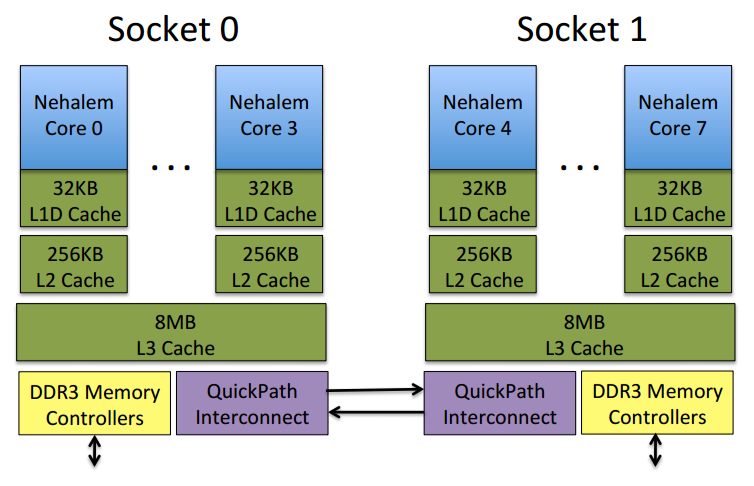
\includegraphics[height=45mm]{images/hardware}
\captionof{figure}{Hardware configuration for experiments.\label{fig:cores}}
\end{center}

\subsection{Problem Solving}

In order to solve the problems listed in Section~\ref{sec:problem}, the authors
conducted experiments in the configuration as explained above. Without going into all of the 23
experiments performed, we can state that the authors successfully investigated the following.
What affects different thread isolation has was investigated by isolating different JVM threads
from the application threads. What affects different thread isolation at the start of execution
was investigated by isolating different JBM thread types at execution startup. All of the
aforementioned isolation occurred on garbage collection, compilation, and all JVM threads
while being isolated on cores and whole sockets. What affects clock frequency had on different
threads was investigates by a combined result of the above. This means threads were isolated all
the time or just at execution startup while the clock frequency of the whole socket was lowered
or raised. (This had to be done at socket level due to hardware limitations, so any isolation
at the core level was not entirely possible for these tests.) 

\subsection {Discussion}

Overall the methodology of this paper was quite sound. They used 23 different experiments to
cover most if not all bases that were presented by their exploratory research areas (listed above).
They laid out each experiment is a very understandable way, first by giving the specific circumstances
of the next experiments followed by the results (always displayed in bar charts), overall findings, as
well as a discussion of said finding. The authors ended up with 14 findings from their 23 experiments
(some were not overly unique) which should be considered a large amount. Since their research question
was more of an exploration into a field with no prior knowledge, it is hard to say that they missed
this or that. However, given their results after the 23 experiments, we would have liked to have seen
a combined effort to pick and choose the best improvements in execution time in order to create
only final test of all possible speed up that were found in order to give a real strong recommendation
in the end of the paper. We would have also liked to have seen more high frequency clock tests as most
of their experiments (except 1) only dealt with lower clock speeds. These extra tests would have 
provided a better frame of reference for the results and findings in comparison.
Other than this, the methodology was great as well as the writing gave great
explanations of the work being performed.


\section{Discussion of Results}
The paper had some clear, well defined and well presented results.  Since the authors used a two-socket system, shown in figure~\ref{fig:cores}, they were able to many isolation tests between sockets.  The paper performed 23 experiements with 14 findings, below we outline some of the most interesting findings, and our opinions:

\subsection{Isolating garbage collection threads to a separate socket}
 
The authors found that this leads to ``small performance degradation (no more than 17\%) for most benchmarks because of increased latency between sockets; however, one benchmark substantially benefits (66\%) from increased cache capacity."

This is interesting because if they separate the GC onto a different socket, if the process has a lot of cache allocation then we will see a large increase in efficiency, conversely, if the application must collect frequently then this will show a large degradation.  This finding would be good to keep in mind for applications similar to ``avrora'', one of their test projects which is sensitive to thread-core mapping.

\subsection{Isolating all threads or compilation thread to one socket in a power-constrainged environment}

The authors find ``When power-constrained in a multi-socket en- vironment, it is better to either keep application and JVM service threads on one socket, and power down the other socket(s), or to isolate the compilation thread onto the sec- ond socket and lower its frequency''. This is a really interesting stat, for two reasons.  The first reason is that if you are building an application with power-constraints, then these are definite possible thread-core mappings that are relevent, and secondly, it would be interesting to compare each one of these methods separately and find the best fit for the application.  

\section{Experiments}

The experiments done were methodological and well documented, however they had some limitations.  From the paper ``...on this machine, it is only possi- ble to change the frequency at a socket-level'' which means that the results are missing out on a lot of added complexity and potential fine tuning that could occur.  

\section{Recommendations}
The authors had a great theme of focusing on performance as a function of the power used, although they should have kept more along this theme, as well, we believe that there should be more integration of findings.  For example, they have some excellent findings that say that we should have isolate the compilation thread to a socket when in a power-constrained environment, but what if we modify the parameters of either of those sockets, what is the net effect.

This paper had a great mix of experiments, but the 

\section{Appendix}


\bibliographystyle{IEEEtran}
\balance
\bibliography{paper}


% End of the paper
\end{document}
